\documentclass[pdftex,11pt,letter]{article}
\usepackage{appendix} %http://www.tex.ac.uk/cgi-bin/texfaq2html?label=appendix
\usepackage{cancel}
\usepackage{amsmath,amssymb,latexsym,float,epsfig}
\usepackage{framed,color,url,fancybox,fullpage,booktabs,subfigure,wrapfig,chngpage,setspace}

\usepackage{amsfonts,caption}
\usepackage{hyperref}
\usepackage{graphicx}
\usepackage{color,epsfig}
\usepackage{bm}
\usepackage{enumerate}
\usepackage{amsmath, amssymb, graphics, setspace,mathtools}
\usepackage{float}
\usepackage[section]{placeins} % places floats within the section
\usepackage[superscript]{cite}


\newcommand{\ssection}[1]{\section[#1]{\centering\normalfont\scshape #1}}
\newcommand{\ssubsection}[1]{\subsection[#1]{\raggedright\normalfont\itshape #1}}
\newcommand\norm[1]{\left\lVert#1 \right\rVert}
\newcommand{\e}{\mathrm{e}}
\newcommand{\pderiv}[2]{\frac{\partial #1}{\partial #2}}
\numberwithin{equation}{section}
\numberwithin{figure}{section}
\usepackage{epstopdf,fancyvrb,cite,hyperref,jvlisting}
%\usepackage[options]{mcode}

\usepackage{pdflscape}%http://texblog.org/2007/11/10/landscape-in-latex/

\newcommand{\ul}[1]{\underline #1}

% Define commands 
\newcommand{\half}{\ensuremath{\frac{1}{2}}}
\newcommand{\bea}{\begin{eqnarray}}
\newcommand{\eea}{\end{eqnarray}}
\newcommand{\beq}{\begin{equation}}
\newcommand{\eeq}{\end{equation}}
\newcommand{\bdm}{\begin{displaymath}}
\newcommand{\edm}{\end{displaymath}}

\newcommand{\etal}[0]{{\em et al.}}
\newcommand{\etc}[0]{{\em etc.}}
\newcommand{\ie}[0]{{\em i.e.,}}


\newcommand{\pd}[2]{\dfrac{\partial #1}{\partial #2}}
\newcommand{\pf}[2]{\dfrac{d #1}{d #2}}
\newcommand{\pdt}[2]{\dfrac{\partial^2 #1}{\partial #2^2}}
\newcommand{\pft}[2]{\dfrac{d^2 #1}{d #2^2}}
\newcommand{\pdtno}[2]{\dfrac{\partial^2 #1}{\partial #2}}
\newcommand{\pdd}[3]{\dfrac{\partial^2 #1}{\partial #2 \partial #3}}
\newcommand{\pff}[3]{\dfrac{d^2 #1}{d #2 d #3}}


\renewcommand\floatpagefraction{0.99}
\renewcommand\topfraction{0.99}
\renewcommand\bottomfraction{0.99}
\renewcommand\textfraction{0.0}

\usepackage{titling}
\setlength{\droptitle}{-1in}   % This is your set screw

% For \url{SOME_URL}, links SOME_URL to the url SOME_URL
\providecommand*\url[1]{\href{#1}{#1}}
% Same as above, but pretty-prints SOME_URL in teletype fixed-width font
\renewcommand*\url[1]{\href{#1}{\texttt{#1}}}

% For \email{ADDRESS}, links ADDRESS to the url mailto:ADDRESS
\providecommand*\email[1]{\href{mailto:#1}{#1}}

\usepackage[superscript]{cite}

\title{\textbf{\textsc{TASS}: A Toolkit for Aircraft Sizing and Synthesis}}
\author{Komahan Boopathy~~\url{komahan@gatech.edu}} \date{\today}
\begin{document}

\maketitle
\vspace{-0.25in}
\rule{\linewidth}{2pt}

\begin{abstract}
A  \ul{T}oolkit for \ul{A}ircraft \ul{S}izing and \ul{S}ynthesis (TASS), capable of performing sizing and synthesis calculations  in the context of conceptual design of aircraft is developed in Matlab\cite{MATLAB}. TASS implements energy-based constraint and weight fraction approach for the mission sizing analyses and provide the user with a design point that is a function of \emph{thrust-weight ratio} and \emph{wing-loading}.  The performance of TASS is benchmarked against the known metrics of a transonic jet fighter aircraft F-86L Sabre (Sabrejet).
\end{abstract}

\section{Introduction and Motivation}

Design of aircraft is subject to tens of thousands of constraints that span across a variety of disciplines such as aerodynamics, structures, controls and performance\cite{NicolaiText,FieldingText,HoweText,RaymerText}. Examples of such constraints, to name a few are: achieving a long cruise range, minimizing the take-off distance, fuel-efficient engines, stealth capabilities for reconnaissance and so on. These constraints are indeed the ones that drive the design and play a pivotal role in shaping the end-design. There has been an increased interest in exploring more at initial stages of design to identify conventional as well as non-conventional configurations -- a strategy that helps one to get a better insight of potential configurations that can meet the design requirements and eliminate restrospective changes that may be due at later stages in design process, that are known to be prohibitively expensive. 
\\\\
Similar motivations have led to the development of tools that ably perform conceptual analysis in various platforms\cite{Raymer2004, Kroo2005}. To this end, this work too aims to develop a toolkit in Matlab\cite{MATLAB} known shortly as TASS, that performs some of the very early phases of aircraft design \ie~the sizing and synthesis. The scope of the current work is limited to the conceptual design phase of aircraft design; more advanced phases in aircraft design (preliminary, detailed design \etc) fall beyond the scope of the current work. Nevertheless, modularity is a key consideration in the development of the toolkit, which enables further advancements a function of time.
\\\\
Energy based constraint analyses form an attractive way to start with aircraft design. The main advantage of energy-based approach over conventional approaches is that it employs Lagrangian paradigm of mechanics, as opposed to Newton's world of vector mechanics. The key idea is that aircraft is treated as a system that converts energy from one form to another as the mission progresses. For example, combustion in the engines convert the chemical energy of the fuel into thermal energy, which in-turn accelerates the gases to rotate the turbines to provide mechanical energy to sustain motion. It is easier to think in terms of scalars such as kinetic energy (depends on velocity) and potential energy (depends on position), compared to resolving forces (e.g. lift, thrust) in along different directions (e.g. vertical, horizontal). Due to these advantages, \textsc{TASS} preferably employs energy based constraint analyses. The mathematical and physical models used in individual disciplines are explained as and when they are introduced in later sections and are not explained here in the spirit of brevity.
\\\\
This report is organized as follows. Section~\ref{theory} outlines the mathematical models behind the aircraft sizing and synthesis procedure. Section~\ref{requirements} outlines the functionality that is expected from the toolkit. Section~\ref{installandbenchmnark} contains detailed step-by-step instructions on the working of the tool with the help of an example. Section~\ref{conclusion} concludes the report highlighting the key aspects of the tool and lays-out scope for further improvements to the toolkit. 


\section{Getting Started}\label{layout}
This section is devoted to provide a high-level overview of the of the software.

\subsection{Installation}
TASS uses native Matlab code for all of its functionality -- including initialization, iterative calculations and graphics, therefore a working version of Matlab\cite{MATLAB} is sufficient. The software is tested to work on both UNIX and Windows based workstations. The source code can be obtained by using \texttt{git clone https://github.com/komahanb/tass.git} from a \textit{terminal} or \textit{shell} program or by downloading \texttt{tass-master.zip} file and extracting it in a working folder of convenience. 

\subsection{Input Layout}
A Graphical User Interface (GUI) is designed to collect all the mission-specific inputs that the user supplies to the software. From an user-standpoint these input parameters are decided based on the complete break-down of mission requirements (e.g. humanitarian, rescue, military missions). Table~\ref{inputs} presents the typical inputs that the user is expected to provide to the software. 

\subsection{Output Layout}
Output layout contains a collection of information interms of values and plots that the user can get from the software.  TASS provides  a constraint analysis plot and enables the user to directly identify a design point in terms of thrust to weight ratio and wing loading. It also provides a mission analysis for the sizing of the system indicating the converged estimated weight and weight contributions from the different weight groups. The following is a comprehensive list of values, tables and plots that TASS is able to present to the user.

\section{Benchmarking TASS}
A brief introduction of the concept under study and a summary of the mission and requirements are  outlined next\cite{MavrisNotes}. The design produced by TASS will be compared to the design of the actual aircraft.

\subsection{Aircraft Requirements}\label{requirements}
 The conceptual design process begins with a defined set of requirements. These requirements lay-out specific constraints and design goals that the end-system must be capable of achieving.  These goals and constraints are often presented the form of Request for Proposal (RFP). %RFP for the fighter is given in Appendix~\ref{}. 

\subsubsection{Functional Requirements}
The functional requirement of the aircraft is to carryout a military mission, which is:
\begin{itemize}
\item to carry a crew member weighing  $210~lbs$ 
\item to carry a payload of $432~lb$
\end{itemize}

\subsubsection{Performance Requirements}
Table~\ref{tab:requirements} breaks-down the performance requirements of the aircraft to be designed using the TASS. 

\begin{table}[h]
\caption{Requirements of the fighter aircraft and for different stages in the mission profile}
\centering 
\begin{tabular}{c| c| c}
\hline\hline
{Segment} & Phase       & Performance Requirements \\
\hline\hline
0-1 	& Takeoff 	& Distance $4400~ft$ \\
	&		& Clear obstacle at $50~ft$\\
	& 		& Maximum power with afterburners\\
	& 		& Air speed $1200~ft/s$ \\
	&		& Sea level runway at $90~F$\\
	&		& Maximum rate of climb $90~ft/s$\\
\hline
1-2	& Climb		& Altitude 35400~ft \\
	& 		& Full military power without afterburners\\
	&		& Maximum rate of climb $90~ft/s$\\
\hline
2-3 	& Cruise climb	& Altitude 38700~ft \\
	&		& Distance 550 nautical miles \\
	&		& Cruise speed 458 knots\\
	&		& Normal power \\
\hline
3-4 	& Loiter	& Altitude 38700 ft\\
	&		& 10 minutes loiter \\
	& 		& normal power\\
\hline
4-5	& Climb		& Altitude 47550 ft\\
\hline
5-6	& Combat 	& Maximum power with afterburners \\
	&		& Duration 5 minutes \\
	& 		& Speed 536 knots \\
\hline
6-7	& Cruise 	& Altitude 37000 ft\\
	& 		& Distance 550 nautical miles\\
	&		& Normal power\\
\hline
7-8	& Loiter	& 10 minutes  \\	
	& 		& Altitude 35000 ft\\
	&		& Maximum endurance conditions \\
\hline
8-9	& Landing	& Distance 5000 ft \\
	&		& Without highilift devices\\	
	&		& 10$\%$ fuel reserve\\
\hline\hline
\end{tabular}
\label{tab:requirements}
\end{table}


\section{Architecture of the Toolkit}\label{theory}
This section provides an outline of the theory, physical and mathematical models used in TASS. A rather comprehensive discussion on these topics can be found in the literature\cite{MattinglyText,NicolaiText,FieldingText,HoweText,RaymerText}. Figure~\ref{fig:sizing_overview} provides a generic overview of the elements involved in the sizing and synthesis process. As it can be seen, \emph{constraint analyses} and \emph{weight estimations} are pivotal in producing the design.  All the discussions in this section are organized in terms of the benchmarking test case Sabrejet F-86 L described in Section~\ref{requirements}.

\begin{figure}[h!]
	\centering
	\includegraphics[scale=0.85]{figures/sizing_overview.pdf}
	\caption{A top level overview of sizing and synthesis process implemented in TASS\cite{MavrisNotes}.}
	\label{fig:sizing_overview}
\end{figure}

\subsection{Standard Atmosphere Model}
TASS has offers the flexibility to choose between two popular standard atmosphere models to the users:
\begin{enumerate}[(a)]
\item U.S. Standard Atmosphere model\cite{US}
\item  Committee on Extension to the Standard Atmosphere (COESA) model\cite{US}
\end{enumerate}
These models are used to obtain the temperature, speed of sound (Mach number), pressure and density as a function of height in the calculations. The default model used in the tool is the U.S. Standard Atmosphere model.

\subsection{Mattingly Energy Equation}

The performance constraints and requirements are set as functions of \emph{thrust loading} (thrust-to-weight ratio) and \emph{wing loading}, the two sizing parameters that contain key information about the top level characteristics of the system\cite{MattinglyText}. The Mattingly Master Enerygy equation is:
\beq\label{eq:energy}
\dfrac{T_{SL}}{W_{TO}} = \dfrac{\beta}{\alpha} 
\left\{ \dfrac{qS}{\beta W_{TO}}
\left[ K_1
\left(
      \dfrac{n\beta W_{TO}}{qS}
\right)^2 
+
K_2
\left(
  \dfrac{n\beta W_{TO}}{qS}
\right) +
C_{D_{0}}
+
\dfrac{R}{qS}
\right]
+
\dfrac{1}{V} \dfrac{d}{dt} \left( h + \dfrac{V^2}{2g_0}\right)
\right\}
\eeq
Table~\ref{tab:param_energy} contains a short definition of the parameters in Eq.~\ref{eq:energy}. 
\begin{table}[h]
\caption{Parameters in Mattingly Energy Equation}
%\medskip
\centering 
\begin{tabular}{c c c c}
\hline\hline
 {Parameter} & Description & English Unit & SI Unit\\
\hline\hline
$T_{SL}$ & sea-level thrust           & lb       & N     \\
$W_{TO}$ & take-off gross weight      & lb       & N     \\  
$q$     & dynamic pressure           & $lb/ft^2$& $N/m^2$\\ 
$S$     & wing planform area         & $ft^2$   & $m^2$  \\   
$C_{D_0}$& drag at zero lift          &  no unit & no unit\\
$K_1$   &                            &          &        \\
$K_2$   &                            &          &        \\
$q$     & load factor                & no unit &  no unit\\ 
$R$     &                            &          &        \\
$V$     &  velocity(speed)           &  $ft/s$  & $m/s$  \\
$h$     &  altitude from sea level   & $ft$     & $m$    \\
$g_0$   &  gravity at sea level      & $ft/s^2$ & $m/s^2$\\
$\alpha$&                            &          &        \\
$\beta$ & instantaneous weight fraction           &          &        \\
\hline
\end{tabular}
\label{tab:param_energy}
\end{table}

\subsection{Constraint Analysis}
By manipulating Eq.~\ref{eq:energy} various constraints pertaining to the mission can be derived. Detailed derivation and treatment of such constraints can be found in Mattingly~\etal\cite{MattinglyText}.

\subsubsection{Constant Altitude/Speed Cruise}

\subsubsection{Constant Speed Climb}

\subsubsection{Constant Altitude/Speed Turn}

\subsubsection{Horizontal Acceleration}

\subsubsection{Takeoff Ground Roll (lots of Thrust)}

\subsubsection{Takeoff Ground Roll (not so much Thrust)}

\subsubsection{Braking Roll}

\subsubsection{Service Ceiling}

\subsection{Weight Estimation}

The  takeoff gross weight $W_{TO}$ can be estimated using
\beq\label{eq:takeoff_weight}
W_{TO} = W_C + W_P +W_E +W_F
\eeq
where $W_C$ is the crew weight, $W_P$ is the payload weight, $W_E$ is the empty weight and $W_F$ is the fuel weight. The design is to be done to carry a crew member who weighs $210~lbs$ and  a payload of $432~lbs$. It is rather difficult to estimate the empty and fuel weight compared to the other counterparts.


\section{Conceptual Design of the Benchmark Fighter}
The comparison of the design obtained using the tool with known configuration of the aircraft follows next. Table~\ref{validation} presents the performance parameters that are calculated using the tool with that of the existing data\cite{}. A good agreement between values demostracte the accuracy of the tool.

\subsection{Perturbations of Constraints}

A good end-result of the conceptual design phase is to identify answers to the following questions? 
\begin{enumerate}
\item Will it work?
\item What does it look like?
\item What requirements drive the design?
\item What tradeoffs should be considered?
\item What should it weigh and cost?
\end{enumerate}

%\subsection{Mission Analysis}
%\subsection{Conceptual Design}

\section{Summary}\label{conclusion}

This work presented a generic toolkit that performs sizing and synthesis of the aircraft configurations at the conceptual design level. The toolkit is provided with a graphical user-interface that helps non-expert users to simulate different requirements at the same time. It is validated against a known configuration of F-86 Sabrejet. 

\bibliography{KomahannoVol}
\bibliographystyle{plain}	

\appendix
\section{RFP for Benchmarking Test Case}\label{rfpbench}

\section{Flexibility of the Tool}
\label{appendix:flexibility}

\subsection{Versatility of the Tool}

\begin{enumerate}

\item The Graphical User Interface (GUI) takes the set of inputs and perform the analyses. As long as the inputs specified are within the validity of the underlying mathematical models, the tool will work for any set of requirements as explained in Section~\ref{benchmarking}.

\item TASS can operate with both English and SI units

\item TASS employs interpolations and extrapolations whenever it encounters data that are be rather difficult to supply or unavailable (e.g.) 

\end{enumerate}

\subsection{Challenges and Cons}

\begin{enumerate}

\item  Since it is extremely laborious to implement sanity checks on the user-supplied values, it is recommended that the users proactively consider the physical meaning of the values supplied (e.g. range, rate of climb)

\end{enumerate}

\end{document}

\begin{figure}[h!]
	\centering
	\includegraphics[scale=0.85]{sizing_overview.pdf}
	\caption{A top level overview of sizing and synthesis process implemented in TASS\cite{MavrisNotes}.}
	\label{fig:sizing_overview}
\end{figure}


predicted takeoff gross weight, T/W, and W/S, calculate the predicted maximum required thrust
at sea level and the predicted wing area. Compare these predicted values to the known values within the Standard Aircraft Characteristics.

\cite{MavrisNotes}
~\cite{NicolaiText}
~\cite{FieldingText}
~\cite{HoweText}
~\cite{RaymerText}
~\cite{Raymer2004}

layout
graphs of interest
scroll bars -- things happen
user interface
clean figures

% add janes world aircraft to citations
%http://www.boeing.com/boeing/history/bna/f86.page>
%Roskam, J., Airplane Design: Part I, Preliminary Sizing of Airplanes, Roskam Aviation and Engineering Corporation, Ottawa, Kansas, 1985
% draw mission profile in matlab based on inputs (back burner)

% standard atmosphere model http://www.mathworks.com/help/aerotbx/ug/atmosisa.html
1.) U.S. Standard Atmosphere, 1976, U.S. Government Printing Office, Washington, D.C.

[T, a, P, rho] = atmosisa(height) implements the mathematical representation of the International Standard Atmosphere values for ambient temperature, pressure, density, and speed of sound for the input geopotential altitude.

This function assumes that below the geopotential altitude of 0 km and above the geopotential altitude of the tropopause, temperature and pressure values are held.

2.) Use 1976 COESA model

Committee on Extension to the Standard Atmosphere has the acronym COESA. [T, a, P, Rho] = atmoscoesa(height, action) implements the mathematical representation of the 1976 COESA United States standard lower atmospheric values. These values are absolute temperature, pressure, density, and speed of sound for the input geopotential altitude.

Below the geopotential altitude of 0 m (0 feet) and above the geopotential altitude of 84,852 m (approximately 278,386 feet), the function extrapolates values. It extrapolates temperature values linearly and pressure values logarithmically.


% weight estimation model
% thrust to weight ratio model
% wing loading model
% drag polar model

% Constraint analysis
  % Constant Altitude / Speed Cruise
  % Constant Speed Climb
  %Takeoff Ground Roll
  % Braking Roll
  % Constant Turn
  %Plot these together and get the deign point

%Mattingly [4], and Roskam [6] citation for energy based approach

% 2006-2007 AIAA Graduate Design Competition RFP

\subsection{Mission Definition}
\subsubsection{Mission Profile}
\subsubsection{Mission Parameters}
the preliminary sizing of the aircraft’s take-off weight and empty weight are calculated.
After the initial inputs are entered, the tool varies the take-off weight until the calculated empty weight equals the historical empty weight



\section*{\centering{Nomenclature}}
\begin{minipage}[b]{1.0\linewidth}%\centering
\begin{tabular}{cccc}%@{}lcl@{}
$T_{SL}$ & sea-level thrust           & lb       & N     \\
$W_{TO}$ & take-off gross weight      & lb       & N     \\  
$C_{D_0}$& drag at zero lift          &  no unit & no unit\\
$K_1$   &                            &          &        \\
$K_2$   &                            &          &        \\
$R$     &                            &          &        \\
$V$     &  velocity(speed)           &  $ft/s$  & $m/s$  \\
$q$     & dynamic pressure           & $lb/ft^2$& $N/m^2$\\ 
$S$     & wing planform area         & $ft^2$   & $m^2$  \\   
$h$     &  altitude from sea level   & $ft$     & $m$    \\
$g_0$   &  gravity at sea level      & $ft/s^2$ & $m/s^2$\\
$\alpha$&                            &          &        \\
$\beta$ &  weight fraction           &          &        \\
%\hline
%  \textit{Subscripts} & & \\
%  $(.)_{global}$ && Corresponds to global surrogate\\
%  \textit{Superscripts} & & \\
%  $(.)^{(j)}$   && j-th training point or test candidate\\
\end{tabular}
\end{minipage}


 U.S. Standard Atmosphere, 1976, U.S. Government Printing Office, Washington, D.C.
